% THIS IS AN EXAMPLE DOCUMENT FOR VLDB 2012
% based on ACM SIGPROC-SP.TEX VERSION 2.7
% Modified by  Gerald Weber <gerald@cs.auckland.ac.nz>
% Removed the requirement to include *bbl file in here. (AhmetSacan, Sep2012)
% Fixed the equation on page 3 to prevent line overflow. (AhmetSacan, Sep2012)

\documentclass{vldb}
\usepackage{graphicx}
\usepackage{balance}  % for  \balance command ON LAST PAGE  (only there!)


\begin{document}

% ****************** TITLE ****************************************

\title{IOT Traffic Simulation: {\ttlit Predictive Analysis}}
\subtitle{2016 Computer Science Senior Thesis}

% possible, but not really needed or used for PVLDB:
%\subtitle{[Extended Abstract]
%\titlenote{A full version of this paper is available as\textit{Author's Guide to Preparing ACM SIG Proceedings Using \LaTeX$2_\epsilon$\ and BibTeX} at \texttt{www.acm.org/eaddress.htm}}}

% ****************** AUTHORS **************************************

% You need the command \numberofauthors to handle the 'placement
% and alignment' of the authors beneath the title.
%
% For aesthetic reasons, we recommend 'three authors at a time'
% i.e. three 'name/affiliation blocks' be placed beneath the title.
%
% NOTE: You are NOT restricted in how many 'rows' of
% "name/affiliations" may appear. We just ask that you restrict
% the number of 'columns' to three.
%
% Because of the available 'opening page real-estate'
% we ask you to refrain from putting more than six authors
% (two rows with three columns) beneath the article title.
% More than six makes the first-page appear very cluttered indeed.
%
% Use the \alignauthor commands to handle the names
% and affiliations for an 'aesthetic maximum' of six authors.
% Add names, affiliations, addresses for
% the seventh etc. author(s) as the argument for the
% \additionalauthors command.
% These 'additional authors' will be output/set for you
% without further effort on your part as the last section in
% the body of your article BEFORE References or any Appendices.

\numberofauthors{2} %  in this sample file, there are a *total*
% of EIGHT authors. SIX appear on the 'first-page' (for formatting
% reasons) and the remaining two appear in the \additionalauthors section.

\author{
% You can go ahead and credit any number of authors here,
% e.g. one 'row of three' or two rows (consisting of one row of three
% and a second row of one, two or three).
%
% The command \alignauthor (no curly braces needed) should
% precede each author name, affiliation/snail-mail address and
% e-mail address. Additionally, tag each line of
% affiliation/address with \affaddr, and tag the
% e-mail address with \email.
%
% 1st. author
\alignauthor
Neeraj Asthana\\
       \affaddr{University of Illinois at Urbana-Champaign}\\
       \affaddr{Laboratory for Cosmological Data Mining}\\
       \affaddr{Urbana, Illinois}\\
       \email{neeasthana@gmail.com}
% 2nd. author
\alignauthor
Robert J. Brunner\titlenote{Senior Thesis Advisor}\\
       \affaddr{University of Illinois at Urbana-Champaign}\\
       \affaddr{Laboratory for Cosmological Data Mining}\\
       \affaddr{Urbana, Illinois}\\
       \email{bigdog@illinois.edu}
}
% There's nothing stopping you putting the seventh, eighth, etc.
% author on the opening page (as the 'third row') but we ask,
% for aesthetic reasons that you place these 'additional authors'
% in the \additional authors block, viz.
%\additionalauthors{Additional authors: John Smith (The Th{\o}rv\"{a}ld Group, {\texttt{jsmith@affiliation.org}}), Julius P.~Kumquat
%(The \raggedright{Kumquat} Consortium, {\small \texttt{jpkumquat@consortium.net}}), and Ahmet Sacan (Drexel University, {\small \texttt{ahmetdevel@gmail.com}})}
%\date{30 July 1999}
% Just remember to make sure that the TOTAL number of authors
% is the number that will appear on the first page PLUS the
% number that will appear in the \additionalauthors section.


\maketitle

\begin{abstract}
The abstract for your paper for the PVLDB Journal submission.
The template and the example document are based on the ACM SIG Proceedings  templates. This file is part of a package for preparing the submissions for review. These files are in the camera-ready format, but they do not contain the full copyright note.
Note that after the notification of acceptance, there will be an updated style file for the camera-ready submission containing the copyright note.
\end{abstract}




\section{Introduction}

\subsection{Problem Statement}
Traffic congestion and associated effects such as air pollution pose major concerns to people who are on the move. Congestion has increased dramatically during the past 20 years in U.S. cities. During this time, the number of hours lost each year by the average driver to congestion has increased by 300 percent. According to Newsweek, the average United States commuter spends an average of 42 hours stuck in traffic every year, resulting in an estimated 160 billion dollar loss from loss of productivity. Currently, drivers are only informed by current and historical traffic conditions in their area. Additionally, increasing the capacity of the roadways is expensive and, in some areas where land is scarce, is not an option.

\subsection{Proposed Solution}
Many popular methods predict traffic states by aggregating streamed GPS data (coordinates, velocities, and timestamps) of many vehicles. With the recent advances in sensor technology, infrastructure for estimating temperature, pressure, humidity, precipitation, etc. are readily available on roadways and can be used to determine driving conditions. The goal and novelty of our project is to combine streamed GPS traffic estimation algorithms with dynamic road sensor data to accurately predict future traffic states and efficiently advise and direct drivers. We will make use of the time decay model for aggregating stream GPS data suggested in “Aggregating and Sampling Methods for Processing GPS Date Streams for Traffic State Estimation” and include methods to incorporate road sensor data. By using both and current traffic conditions and sensors on the road, we hope to understand how traffic may change on a single road segment in the near future (30 minutes, 1 hour, etc.). 

\begin{figure}
\centering
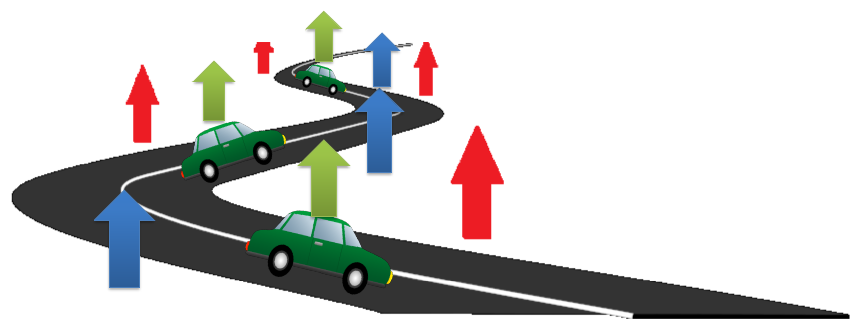
\includegraphics[width=3.5in,height=1.25in]{Road}
\caption{Cars and Sensors along a road segment generating data that can be processed by our system.}
\label{fig:road}
\end{figure}

\section{Data Sources}
There are two major data sources necessary for this project: streamed GPS data and road sensor data. These data sets are continually generated and streamed to our backend clusters and these portions of the project were produced by my fellow project collaborators. Rishabh’s work focused on the generation of streamed GPS data while Vaishali’s work focused on generating road sensor data. 

\subsection{Streamed GPS Data}
There will be many vehicles travelling along the roads of our model and each vehicle will be continuously be emitting data to our backend server at a predefined interval (i.e. every second, every minute, etc.). Each emitted data packet from a vehicle will be of the form (vehicle id, location, velocity, timestamp) which can be abbreviated as ($id, v_i, l_i, t_i$). The vehicle id is a unique identifier for each vehicle. The location consists of a geodesic latitude and longitude coordinate. The velocity field consists of the vehicle’s current velocity which will be measured in meters per second. The timestamp references the time at which the location and velocity data was recorded in the form \%Y-\%m-\%d \%H:\%M:\%S.

\subsection{Streamed Road Sensor Data}
Our model allows us to generalize to any number or type of sensor, however for now we will only focus on a single type of sensor which measures road surface temperature. Sensors will be placed along a roadway at a predefined interval ((i.e. every mile, every five miles, etc.) and I will assume that these locations are known. Each sensor will periodically emit information to our backend server at a predefined interval (i.e. every second, every minute, etc.). Each sensor data packet will be in the form: (sensor id, temperature, timestamp). The sensor id is a unique identifier for each sensor. The temperature defines a road surface temperature at the location of the sensor in Celsius degrees. The timestamp references the time at which the temperature was recorded in the form \%Y-\%m-\%d \%H:\%M:\%S. In the future we will focus on extending our model to incorporate different types of sensors. Other potential sensor types include humidity, wind speed, water precipitation, etc. 

\section{Technical Specifications}
Our backend will be implemented on the NCSA ACX cloud computing cluster. The purpose of these systems is to efficiently stream our data sources to allow for real time traffic state prediction. The focus of this paper will mostly be centered on the stream processing/cloud computing system by implementing the model mentioned in sections below with the data streamed from our message broker. A basic network diagram of the data flow is included in Figure 2 for reference. This section describes each of the systems and explains the actions taken at each step.

\subsection{Network Resources}

\subsubsection{Message Broker (Kafka)}
All vehicle and sensor data will be aggregated and ordered by a single message broker for efficient processing. Large amounts of real time data will continually be streaming into our backend and a message broker like Apache Kafka will help us efficiently manage large amounts of messages. All the data captured at this step will be aggregated and ordered so that it can be sent to the data storage and stream processing units. The Kafka cluster contains two major queues, “traffic” and “weather”, known as topics. The “traffic” topic contains streamed vehicle data and each entry is of the form (latitude, longitude, velocity, time, vehicle id). The “weather” topic contains streamed vehicle data and each entry is of the form (segment id, time, measurement).

\subsubsection{Stream Processing (Spark)}
The most recent data from the cars and the sensors will be sent to this unit to update the current road condition models using the time decay model. The newest data will be streamed into the system and be used (along with historical GPS data from the data store) to generate a new model describing the road conditions. Local variables will be stored on all of the nodes in the Spark Cluster that persist and update the parameters from the time decay model (details about the time decay model are provided in the following section). More details and specific code segments are provided about Spark Streaming are provided in the section below. There are considerations to also use or benchmark Apache Flink or Apache Storm in place of Spark as these may scale better to larger data streams. 

\subsubsection{Database (Cassandra)}
All data will be stored in this unit to either be included in future models or displayed on the front end interface.

\subsection{Data Pipeline}
Figure 3 describes the general flow of the data between different clusters.  Data is generated by the Vehicles and Road Sensors at a specified time interval (i.e. every second, mintute, etc.). This large stream of data is then aggregated and sorted by Kafka, placing the data into two separate streams. The data is then sent to the Web Dashboard to display the current traffic conditions and it is also sent to the Spark Streaming instance to be processed into future speed predictions. The current conditions and predicted speeds are stored in a Cassandra database to be analyzed in depth at a later point. Data is also sent to the Web Dashboard which can then be displayed on consoles in vehicles. 


\begin{figure}
\centering
\includegraphics[width=3.25in,height=1.25in]{NetworkDiagram}
\caption{Network Diagram highlighting the major tasks occuring at each level.}
\label{fig:networkdiagram}
\end{figure}


\section{Time Decay Model}
Our model incorporates the time decay model suggested in “Aggregating and Sampling Methods for Processing GPS Date Streams for Traffic State Estimation” with road sensor data to estimate traffic states on specific road segments. We implement the aggregation based method mentioned in the paper as it requires minimal resources to implement and is efficient at estimating average speeds on road segments. We further adjusted the calculated average speed on each road segment based on data from road sensors from that same road segment. 

The message broker (Kafka) sends vehicle packets of the form (vehicle id, location, velocity, timestamp) and each road sensor sends packets of the form (sensor id, temperature, timestamp), which all will be ordered and aggregated by the message broker to form a stream and sent to the Spark Streaming system. 

\subsection{Velocity Estimation}
Previous models of estimating traffic states from GPS data streams focus on either historical data or a sliding window (SW) sampling method. Historical methods attempt to aggregate previous speeds of vehicles on a particular road (each of which has an equal weight); however this method is not extremely accurate in the short term as GPS data streams are volatile and evolve rapidly based on different circumstances. The sliding-window sampling method conversely saves the most recent GPS data stream and uses only a select few point to estimate new traffic states. This also may not be completely accurate when estimating traffic states as it creates unstable traffic conditions that may not reflect the average behavior of a specific road. Therefore, I plan to implement a time decay model which highly values new data records but also factors old data records. This method is also online and real time, allowing us to process data quickly and return current information. 

The key idea of the time decay model is to weight new records higher than old records in that same location. This is accomplished by weighting each record with a value w using the following exponential decay function where i represents the ith GPS record, t is the processing time, and ti is the timestamp of the current record:

\begin{equation}w(i,t)=e^{\beta(t_i-t)}\end{equation}

where $\beta > 0$ and $t \geq t_i$.

Using this model, our system calculates weights for each of the data records on a specific road segment and older records are weighted less than newer records. 

We must also notice that high velocities are more useful than low velocities as low velocities can signal events that are not related to traffic flow such as parked vehicles or stopping at a red light. Therefore, we must weigh high velocity data as more important than low velocity data which is accomplish by assigning another weight to each record using a function g that is positive, nondecreasing, and monotonic as follows:

\begin{equation}w^v(i)=g(v_i)\end{equation}

Our model then assigns a full weight to a specific GPS data point by the following equation:

\begin{equation}w^*(i,t)=w(i,t) \cdot w^v(i) \end{equation}

For each predefined road segment, defined as \textit{r} (specifying a latitude and longitude radius), the estimated average velocity at time \textit{t} can be found using the following equation:

\begin{equation}\overline{V}(r)=\frac{\sum_{n=1}^{m} f(t_i - L) \cdot g(v_i) \cdot v_i}{\sum_{n=1}^{m} f(t_i - L) \cdot g(v_i)}\end{equation}


\subsection{Model Updates}

Equation 4 would be ideal for a batch processing system, however, it does not scale well to a fully streamed system that must constantly be updated with new values. The model must be easily updated with newly streamed data points as well. In order to accomplish this, we will break $\overline{V}(r)$ into its numerator and denominator and define two new values \textit{X} and \textit{Y}:

\begin{equation}X = \sum_{n=1}^{m} f(t_i - L) \cdot g(v_i) \cdot v_i\end{equation}

\begin{equation}Y = \sum_{n=1}^{m} f(t_i - L) \cdot g(v_i)\end{equation}

The values \textit{X} and \textit{Y} will be persisted for each road segment and new observations can incrementally be added to these specific components. Then, whenver a velocity estimate ($\overline{V}(r)$) is needed, the values can be divided as $\overline{V}(r)=\frac{X}{Y}$.


\subsection{Incorporating Road Sensors}
The model described above is used only to get current estimates of speeds on roads and is not novel. Instead, our model instead incorporates road sensor data from road segments along with the estimated current velocity of those segments to project a future velocity on that same road segment (ex. In the next 30 mins, hour, etc.). Our current model only uses road surface temperatures with known parameters to predict a future speed. However, in the future when multiple sensors are used, we will use a machine learning algorithm (i.e. simple linear ridge regression) to estimate future velocities using all of these sensor data as inputs. 

\begin{figure}
\centering
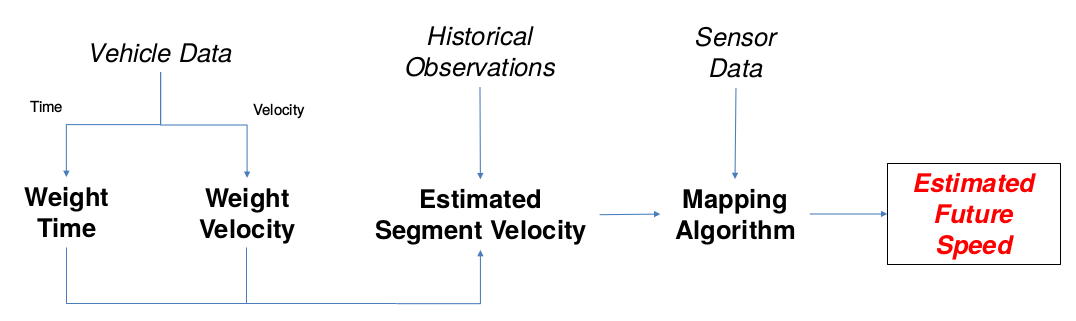
\includegraphics[width=3.25in,height=1.25in]{TimeDecay}
\caption{Describes how data flows through our modified Time Decay model to produce an estimated future speed.}
\label{fig:networkdiagram}
\end{figure}

\section {Dynamic Map Matching Algorithm}
Car data and road sensor data each have locations associated with each observation and must be matched to road segments in order to update specific model parameters. Therefore, we must translate a latitude and longitude observation to a road segment. 

\subsection{Code}
The current algorithm matches a road segment by find the closest road segment to the observation. The algorithm casts a radius of .25 kilometers to accommodate for slight errors in GPS streamed locations. The code contains 2 key functions. The first function (distance) takes two latitude and longitude pairs and calculates the distance between them. The second function attempts to find the closest segment to an observation’s location.

insert code

In the future, we hope to be able to better distinguish between road segments by including a direction of travel field within each observation. In this way, we will be able to accurately match road segments if vehicles are at an intersection or close to another road. We will also be able to keep data for two way traffic (incoming and outgoing for a road segment). 

\subsection{Citations}
Citations to articles \cite{bowman:reasoning, clark:pct, braams:babel, herlihy:methodology},
conference
proceedings \cite{clark:pct} or books \cite{salas:calculus, Lamport:LaTeX} listed
in the Bibliography section of your
article will occur throughout the text of your article.
You should use BibTeX to automatically produce this bibliography;
you simply need to insert one of several citation commands with
a key of the item cited in the proper location in
the \texttt{.tex} file \cite{Lamport:LaTeX}.
The key is a short reference you invent to uniquely
identify each work; in this sample document, the key is
the first author's surname and a
word from the title.  This identifying key is included
with each item in the \texttt{.bib} file for your article.

The details of the construction of the \texttt{.bib} file
are beyond the scope of this sample document, but more
information can be found in the \textit{Author's Guide},
and exhaustive details in the \textit{\LaTeX\ User's
Guide}\cite{Lamport:LaTeX}.

This article shows only the plainest form
of the citation command, using \texttt{{\char'134}cite}.
This is what is stipulated in the SIGS style specifications.
No other citation format is endorsed.

\subsection{Tables}
Because tables cannot be split across pages, the best
placement for them is typically the top of the page
nearest their initial cite.  To
ensure this proper ``floating'' placement of tables, use the
environment \textbf{table} to enclose the table's contents and
the table caption.  The contents of the table itself must go
in the \textbf{tabular} environment, to
be aligned properly in rows and columns, with the desired
horizontal and vertical rules.  Again, detailed instructions
on \textbf{tabular} material
is found in the \textit{\LaTeX\ User's Guide}.

Immediately following this sentence is the point at which
Table 1 is included in the input file; compare the
placement of the table here with the table in the printed
dvi output of this document.

\begin{table}
\centering
\caption{Frequency of Special Characters}
\begin{tabular}{|c|c|l|} \hline
Non-English or Math&Frequency&Comments\\ \hline
\O & 1 in 1,000& For Swedish names\\ \hline
$\pi$ & 1 in 5& Common in math\\ \hline
\$ & 4 in 5 & Used in business\\ \hline
$\Psi^2_1$ & 1 in 40,000& Unexplained usage\\
\hline\end{tabular}
\end{table}

To set a wider table, which takes up the whole width of
the page's live area, use the environment
\textbf{table*} to enclose the table's contents and
the table caption.  As with a single-column table, this wide
table will ``float" to a location deemed more desirable.
Immediately following this sentence is the point at which
Table 2 is included in the input file; again, it is
instructive to compare the placement of the
table here with the table in the printed dvi
output of this document.


\begin{table*}
\centering
\caption{Some Typical Commands}
\begin{tabular}{|c|c|l|} \hline
Command&A Number&Comments\\ \hline
\texttt{{\char'134}alignauthor} & 100& Author alignment\\ \hline
\texttt{{\char'134}numberofauthors}& 200& Author enumeration\\ \hline
\texttt{{\char'134}table}& 300 & For tables\\ \hline
\texttt{{\char'134}table*}& 400& For wider tables\\ \hline\end{tabular}
\end{table*}
% end the environment with {table*}, NOTE not {table}!

\subsection{Figures}
Like tables, figures cannot be split across pages; the
best placement for them
is typically the top or the bottom of the page nearest
their initial cite.  To ensure this proper ``floating'' placement
of figures, use the environment
\textbf{figure} to enclose the figure and its caption.

This sample document contains examples of \textbf{.pdf} files to be
displayable with \LaTeX (See Figures \ref{fig:fly} and \ref{fig:bigfly}).  More details on each of these is found in the
\textit{Author's Guide}.

\begin{figure}
\centering
\includegraphics{fly}
\caption{A sample black and white graphic (.pdf format).}
\label{fig:fly}
\end{figure}

\begin{figure}
\centering
\includegraphics[width=1in,height=1in]{fly}
\caption{A sample black and white graphic (.pdf format)
that has been resized with the \texttt{includegraphics} command.}
\label{fig:bigfly}
\end{figure}


As was the case with tables, you may want a figure
that spans two columns.  To do this, and still to
ensure proper ``floating'' placement of tables, use the environment
\textbf{figure*} to enclose the figure and its caption (See Figure~\ref{fig:flies}). And don't forget to end the environment with {figure*}, not {figure}!

\begin{figure*}
\centering
\includegraphics{flies}
\caption{A sample black and white graphic (.pdf format)
that needs to span two columns of text.}
\label{fig:flies}
\end{figure*}


Note that only {\textbf{.pdf}} files were used; if you want to include
{\textbf{.ps}} or {\textbf{.eps}} formats, you can use the
\texttt{{\char'134}epsfig} or \texttt{{\char'134}psfig}
commands as appropriate for the different file types.

\subsection{Theorem-like Constructs}
Other common constructs that may occur in your article are
the forms for logical constructs like theorems, axioms,
corollaries and proofs.  There are
two forms, one produced by the
command \texttt{{\char'134}newtheorem} and the
other by the command \texttt{{\char'134}newdef}; perhaps
the clearest and easiest way to distinguish them is
to compare the two in the output of this sample document:

This uses the \textbf{theorem} environment, created by
the\linebreak\texttt{{\char'134}newtheorem} command:
\newtheorem{theorem}{Theorem}
\begin{theorem}
Let $f$ be continuous on $[a,b]$.  If $G$ is
an antiderivative for $f$ on $[a,b]$, then
\begin{displaymath}\int^b_af(t)dt = G(b) - G(a).\end{displaymath}
\end{theorem}

The other uses the \textbf{definition} environment, created
by the \texttt{{\char'134}newdef} command:
\newdef{definition}{Definition}
\begin{definition}
If $z$ is irrational, then by $e^z$ we mean the
unique number which has
logarithm $z$: \begin{displaymath}{\log e^z = z}\end{displaymath}
\end{definition}

Two lists of constructs that use one of these
forms is given in the
\textit{Author's  Guidelines}.


There is one other similar construct environment, which is
already set up
for you; i.e. you must \textit{not} use
a \texttt{{\char'134}newdef} command to
create it: the \textbf{proof} environment.  Here
is a example of its use:
\begin{proof}
Suppose on the contrary there exists a real number $L$ such that
\begin{displaymath}
\lim_{x\rightarrow\infty} \frac{f(x)}{g(x)} = L.
\end{displaymath}
Then
\begin{align*}
l&=\lim_{x\rightarrow c} f(x)
= \lim_{x\rightarrow c}
\left[ g{x} \cdot \frac{f(x)}{g(x)} \right ] \\
&= \lim_{x\rightarrow c} g(x) \cdot \lim_{x\rightarrow c}
\frac{f(x)}{g(x)} = 0\cdot L = 0,
\end{align*}
which contradicts our assumption that $l\neq 0$.
\end{proof}

Complete rules about using these environments and using the
two different creation commands are in the
\textit{Author's Guide}; please consult it for more
detailed instructions.  If you need to use another construct,
not listed therein, which you want to have the same
formatting as the Theorem
or the Definition\cite{salas:calculus} shown above,
use the \texttt{{\char'134}newtheorem} or the
\texttt{{\char'134}newdef} command,
respectively, to create it.

\subsection*{A {\secit Caveat} for the \TeX\ Expert}
Because you have just been given permission to
use the \texttt{{\char'134}newdef} command to create a
new form, you might think you can
use \TeX's \texttt{{\char'134}def} to create a
new command: \textit{Please refrain from doing this!}
Remember that your \LaTeX\ source code is primarily intended
to create camera-ready copy, but may be converted
to other forms -- e.g. HTML. If you inadvertently omit
some or all of the \texttt{{\char'134}def}s recompilation will
be, to say the least, problematic.

\section{Conclusions}
This paragraph will end the body of this sample document.
Remember that you might still have Acknowledgments or
Appendices; brief samples of these
follow.  There is still the Bibliography to deal with; and
we will make a disclaimer about that here: with the exception
of the reference to the \LaTeX\ book, the citations in
this paper are to articles which have nothing to
do with the present subject and are used as
examples only.
%\end{document}  % This is where a 'short' article might terminate

% ensure same length columns on last page (might need two sub-sequent latex runs)
\balance

%ACKNOWLEDGMENTS are optional
\section{Acknowledgments}
This section is optional; it is a location for you
to acknowledge grants, funding, editing assistance and
what have you.  In the present case, for example, the
authors would like to thank Gerald Murray of ACM for
his help in codifying this \textit{Author's Guide}
and the \textbf{.cls} and \textbf{.tex} files that it describes.


% The following two commands are all you need in the
% initial runs of your .tex file to
% produce the bibliography for the citations in your paper.
\bibliographystyle{abbrv}
\bibliography{vldb_sample}  % vldb_sample.bib is the name of the Bibliography in this case
% You must have a proper ".bib" file
%  and remember to run:
% latex bibtex latex latex
% to resolve all references

\subsection{References}
Generated by bibtex from your ~.bib file.  Run latex,
then bibtex, then latex twice (to resolve references).

%APPENDIX is optional.
% ****************** APPENDIX **************************************
% Example of an appendix; typically would start on a new page
%pagebreak

\begin{appendix}
You can use an appendix for optional proofs or details of your evaluation which are not absolutely necessary to the core understanding of your paper. 

\section{Final Thoughts on Good Layout}
Please use readable font sizes in the figures and graphs. Avoid tempering with the correct border values, and the spacing (and format) of both text and captions of the PVLDB format (e.g. captions are bold).

At the end, please check for an overall pleasant layout, e.g. by ensuring a readable and logical positioning of any floating figures and tables. Please also check for any line overflows, which are only allowed in extraordinary circumstances (such as wide formulas or URLs where a line wrap would be counterintuitive).

Use the \texttt{balance} package together with a \texttt{\char'134 balance} command at the end of your document to ensure that the last page has balanced (i.e. same length) columns.

\end{appendix}



\end{document}
